\documentclass[11pt]{article}\usepackage[a4paper,margin=22mm]{geometry}\usepackage{graphicx,booktabs,hyperref}\begin{document}\title{Body-fitted finite-volume NACA0012 verification}\maketitle\section{Problem and method}NACA0012, Re=1000, incidence 4 degrees. Domain size and prescribed far-field velocity differ from the reference study. Conforming Gmsh triangles, conservative linear upwind transport, geometric interpolation and Gauss face-pressure integration are verified using raw fields and independent NumPy equation replay. Strict physical errors are below 3\% only for runs explicitly accepted below. Full problem, software commands, references and limits are in report.md.\section{Results}\begin{tabular}{rrrrl}\toprule Cells & Iterations & $C_D$ & $C_L$ & Accepted\\\midrule 3934 & 560 & 0.127569525 & 0.232070235 & False \\
15018 & 1454 & 0.127141246 & 0.216320534 & False \\
\bottomrule\end{tabular}\section{Computed fields and convergence}\begin{figure}[p]\centering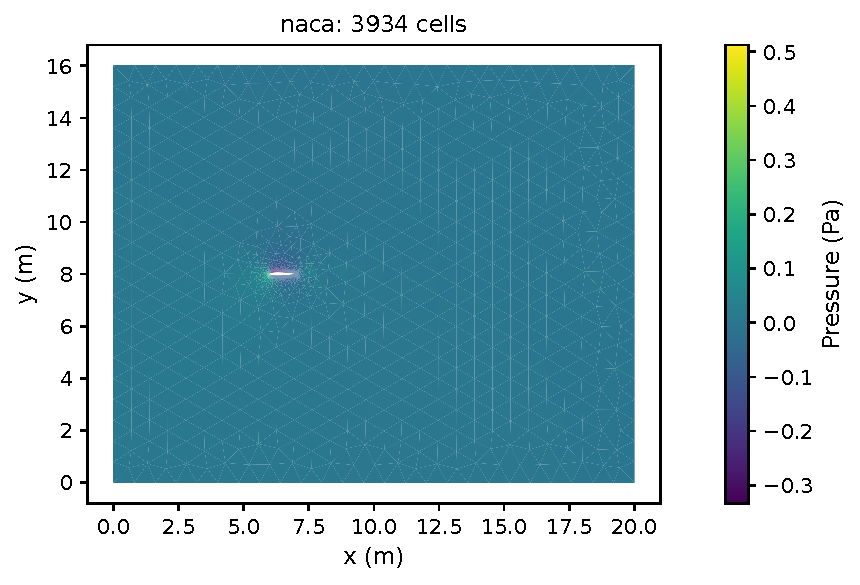
\includegraphics[width=.95\linewidth]{scale-2/figures/pressure-global.pdf}\caption{scale 2 figures pressure global}\end{figure}\begin{figure}[p]\centering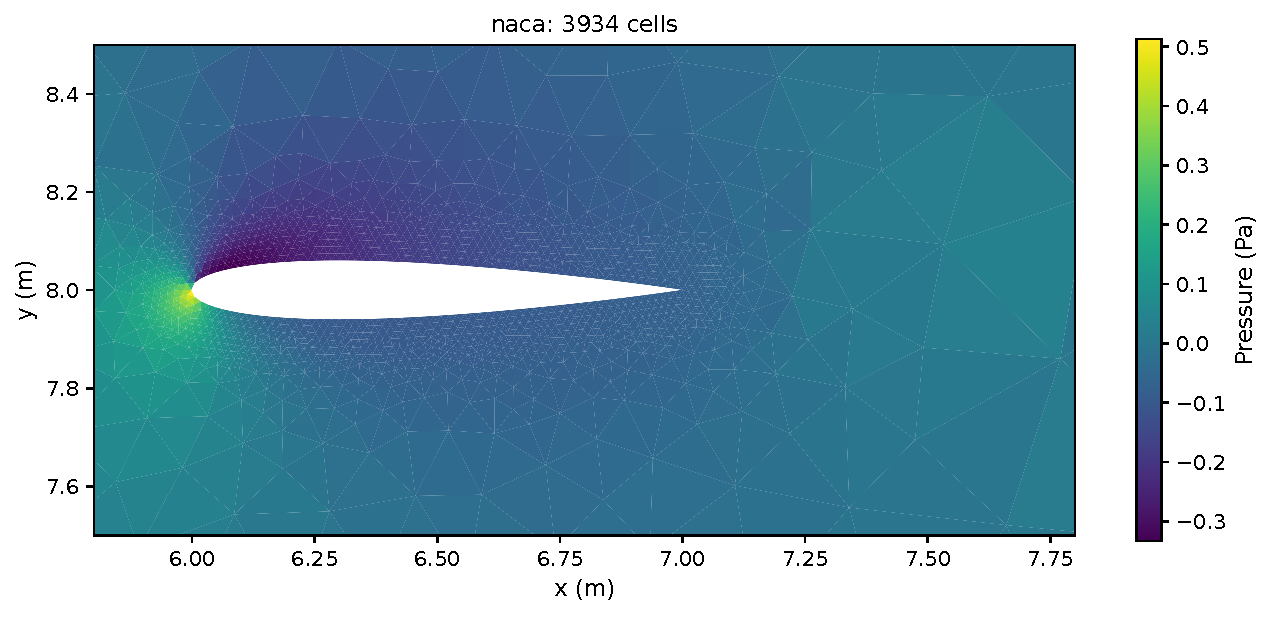
\includegraphics[width=.95\linewidth]{scale-2/figures/pressure-local.pdf}\caption{scale 2 figures pressure local}\end{figure}\begin{figure}[p]\centering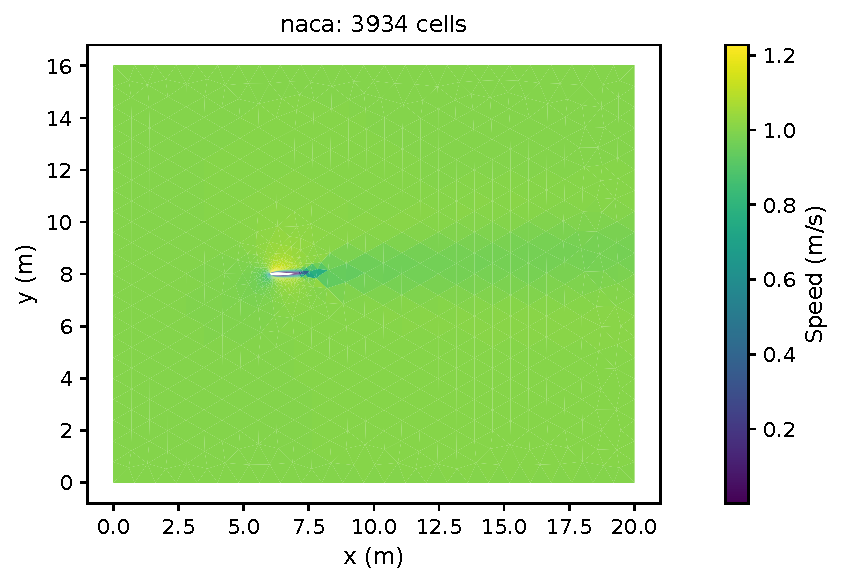
\includegraphics[width=.95\linewidth]{scale-2/figures/velocity-global.pdf}\caption{scale 2 figures velocity global}\end{figure}\begin{figure}[p]\centering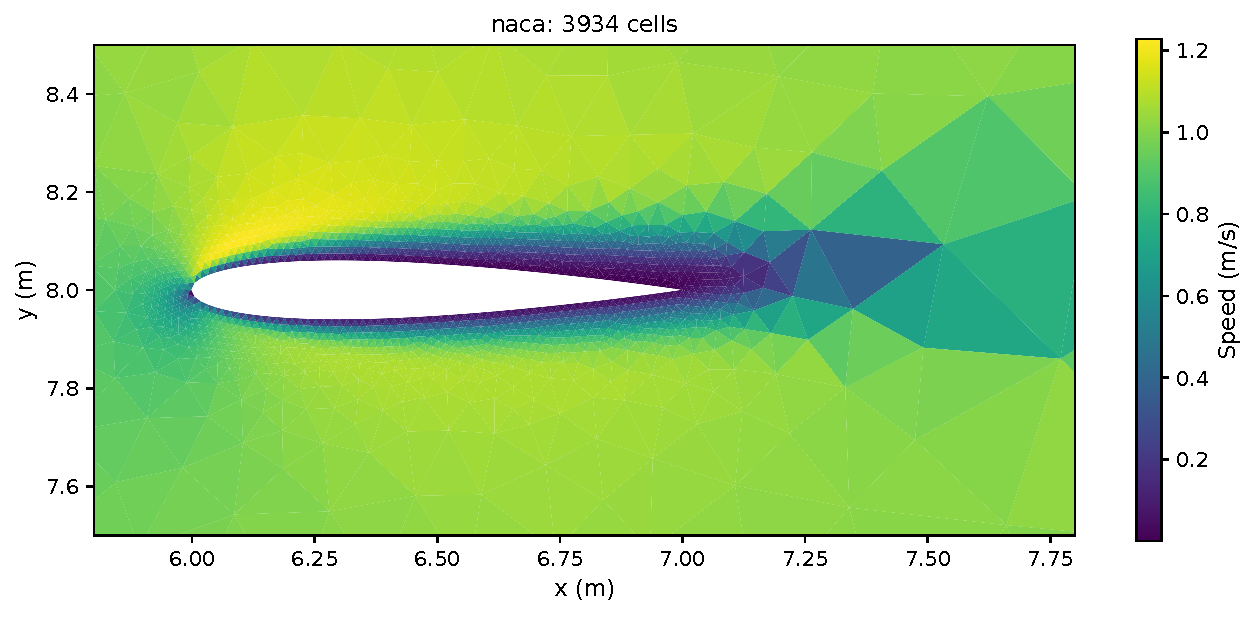
\includegraphics[width=.95\linewidth]{scale-2/figures/velocity-local.pdf}\caption{scale 2 figures velocity local}\end{figure}\begin{figure}[p]\centering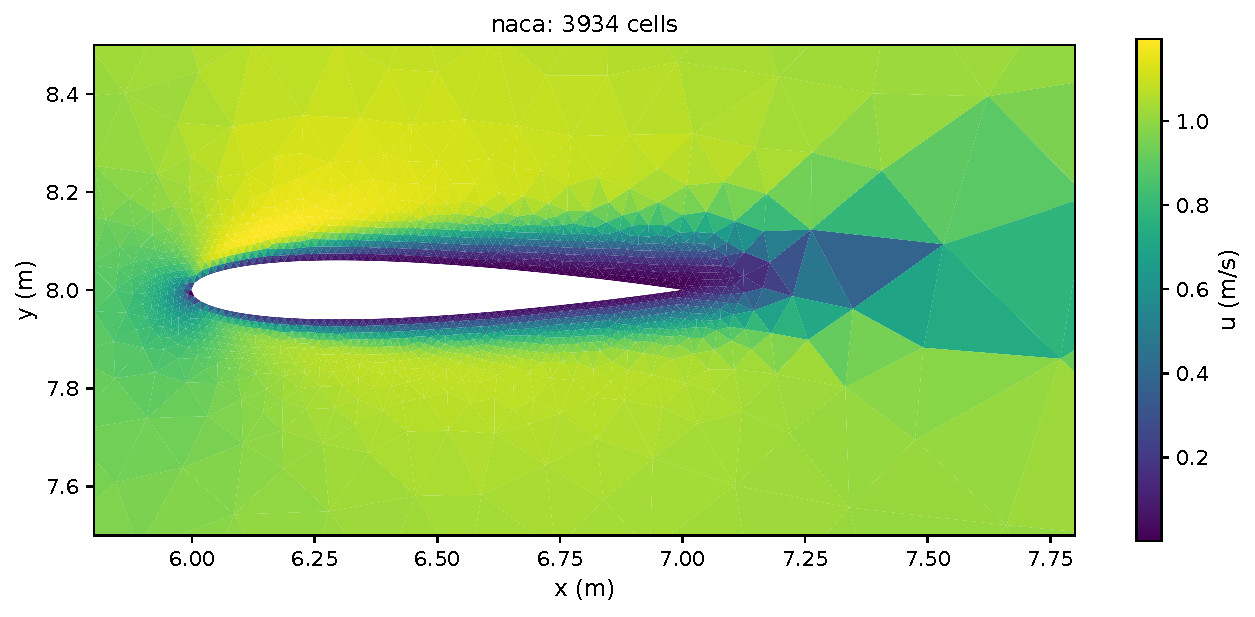
\includegraphics[width=.95\linewidth]{scale-2/figures/u-local.pdf}\caption{scale 2 figures u local}\end{figure}\begin{figure}[p]\centering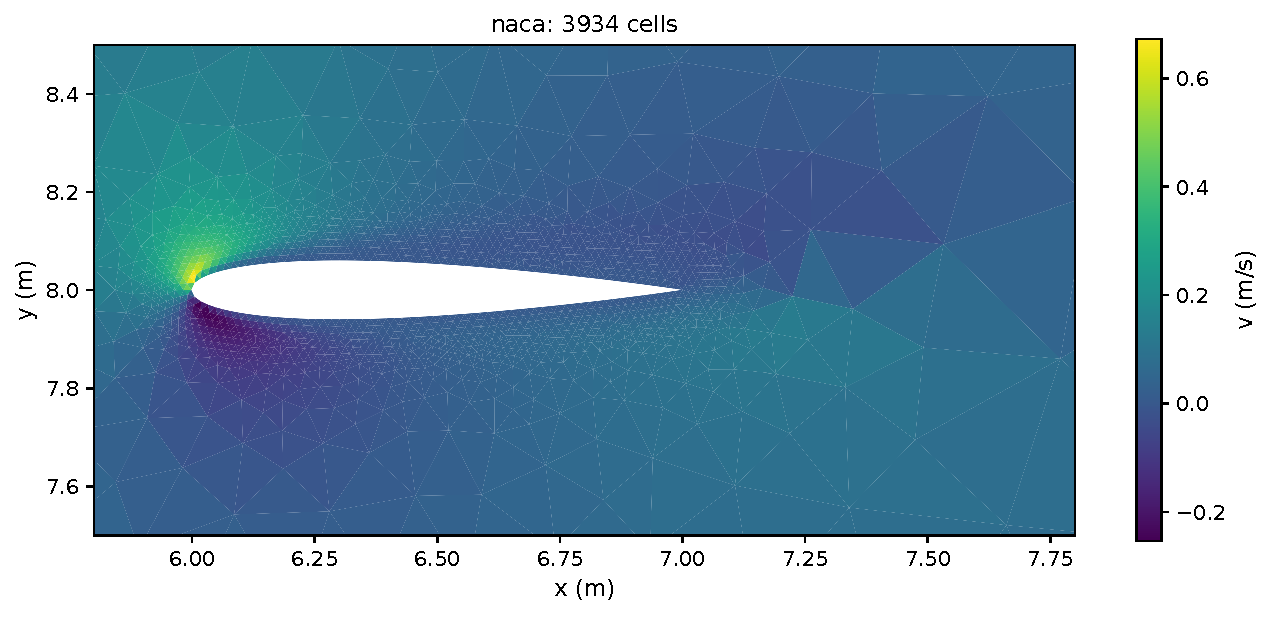
\includegraphics[width=.95\linewidth]{scale-2/figures/v-local.pdf}\caption{scale 2 figures v local}\end{figure}\begin{figure}[p]\centering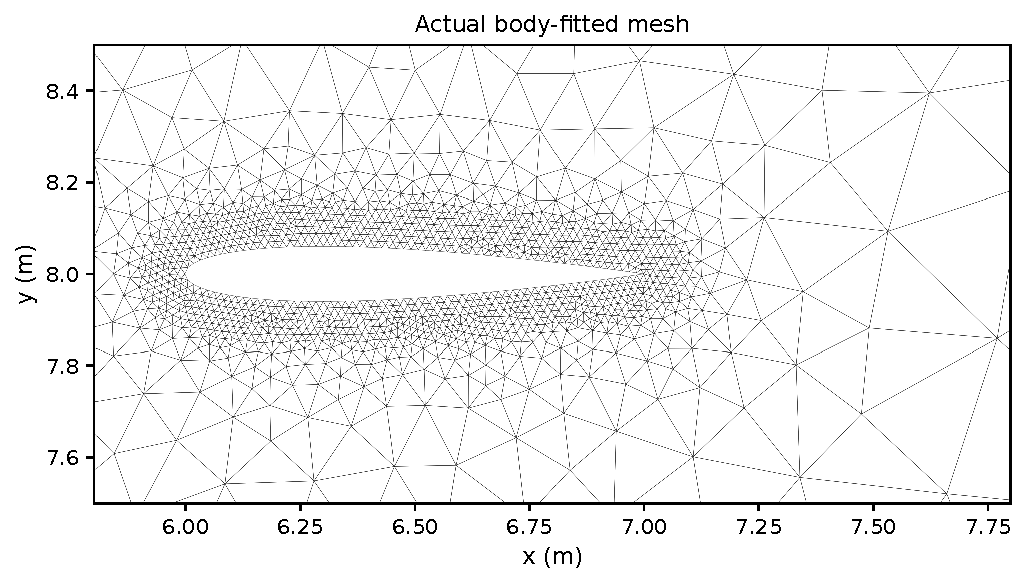
\includegraphics[width=.95\linewidth]{scale-2/figures/mesh-local.pdf}\caption{scale 2 figures mesh local}\end{figure}\begin{figure}[p]\centering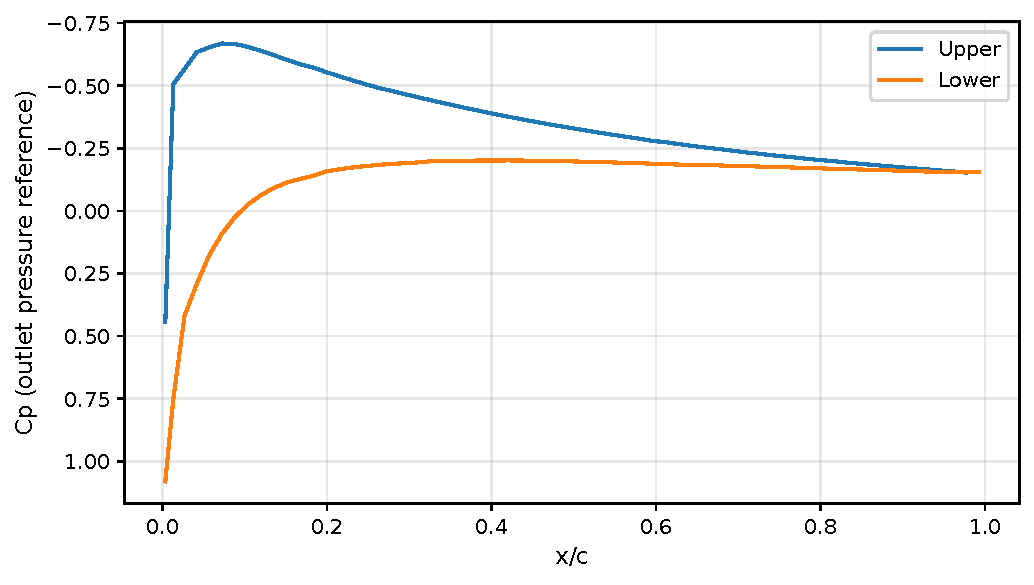
\includegraphics[width=.95\linewidth]{scale-2/figures/surface-pressure.pdf}\caption{scale 2 figures surface pressure}\end{figure}\begin{figure}[p]\centering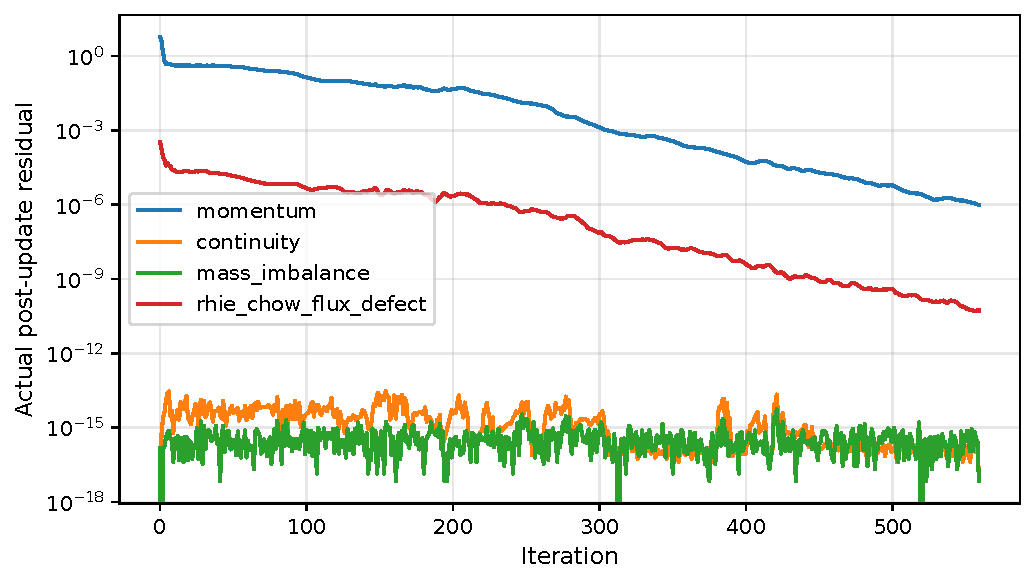
\includegraphics[width=.95\linewidth]{scale-2/figures/residuals.pdf}\caption{scale 2 figures residuals}\end{figure}\begin{figure}[p]\centering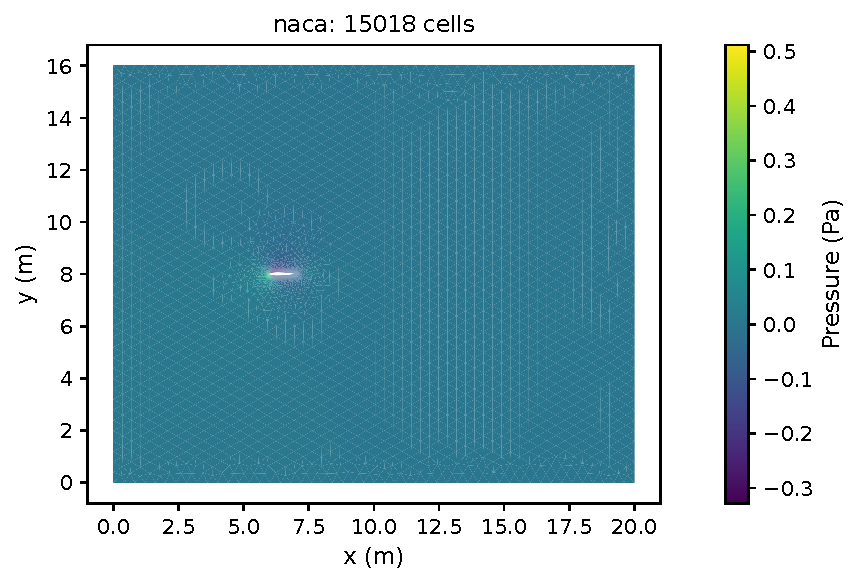
\includegraphics[width=.95\linewidth]{scale-1/figures/pressure-global.pdf}\caption{scale 1 figures pressure global}\end{figure}\begin{figure}[p]\centering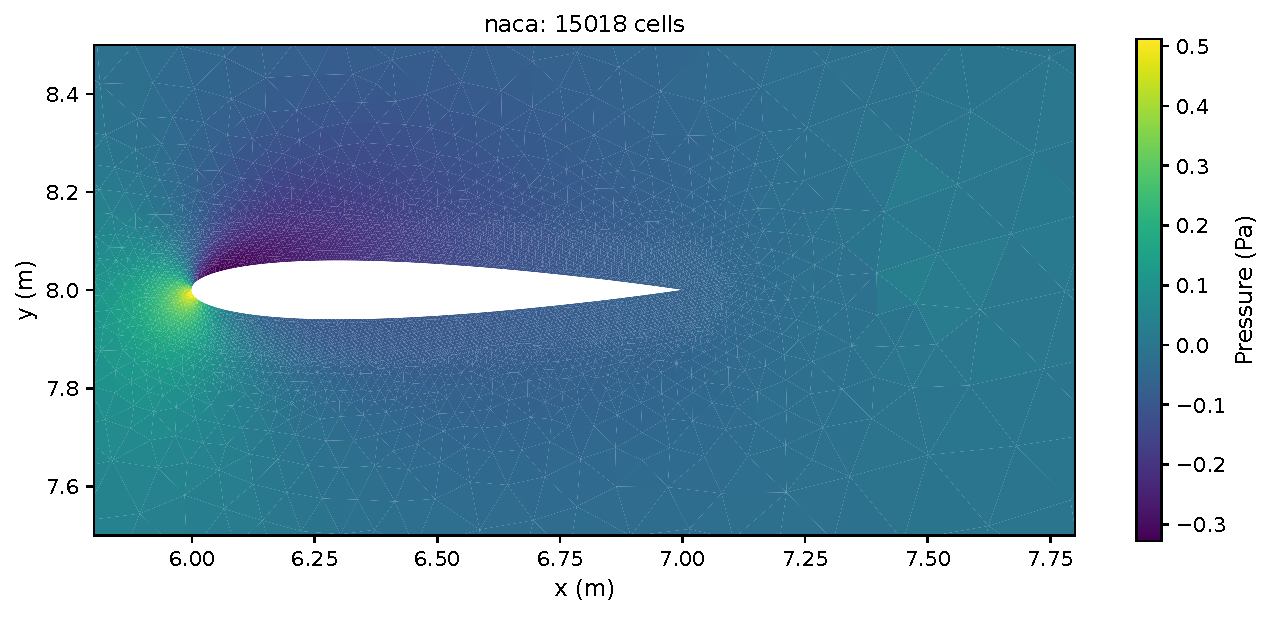
\includegraphics[width=.95\linewidth]{scale-1/figures/pressure-local.pdf}\caption{scale 1 figures pressure local}\end{figure}\begin{figure}[p]\centering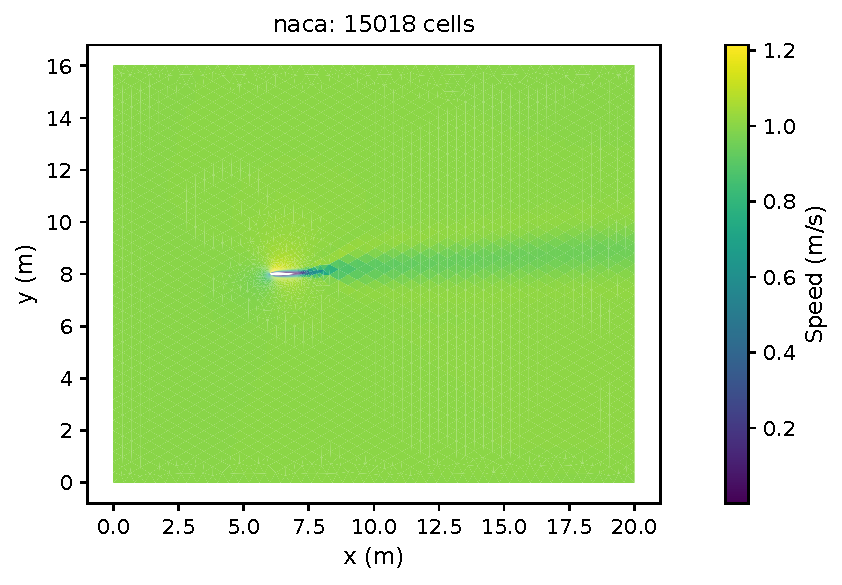
\includegraphics[width=.95\linewidth]{scale-1/figures/velocity-global.pdf}\caption{scale 1 figures velocity global}\end{figure}\begin{figure}[p]\centering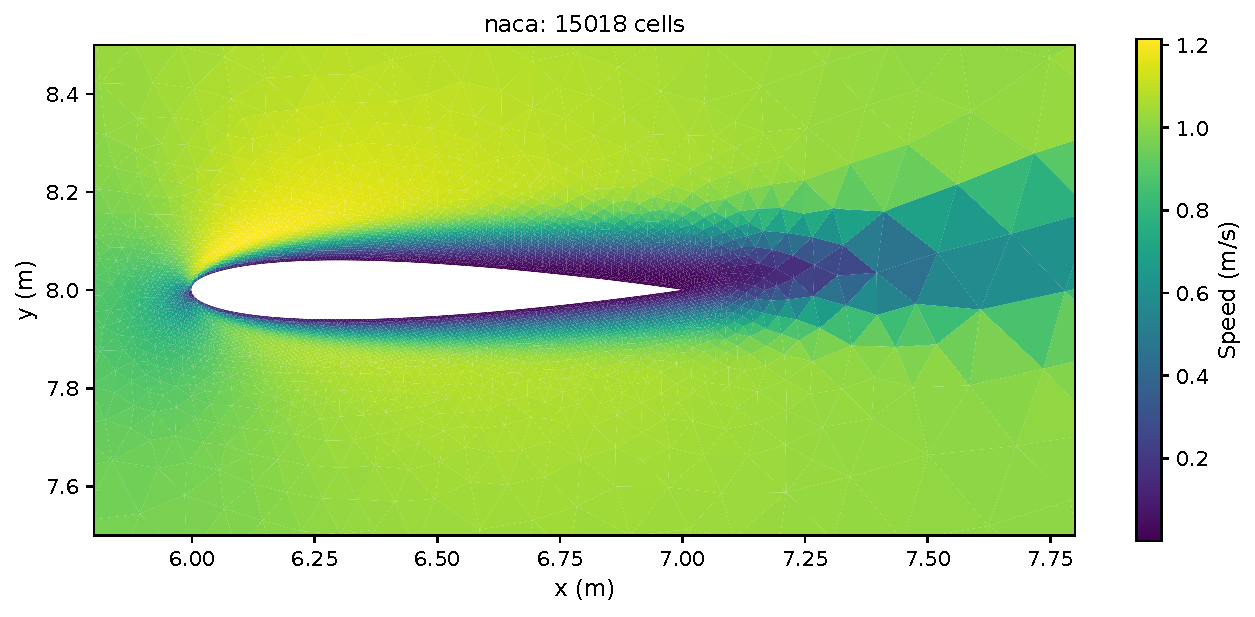
\includegraphics[width=.95\linewidth]{scale-1/figures/velocity-local.pdf}\caption{scale 1 figures velocity local}\end{figure}\begin{figure}[p]\centering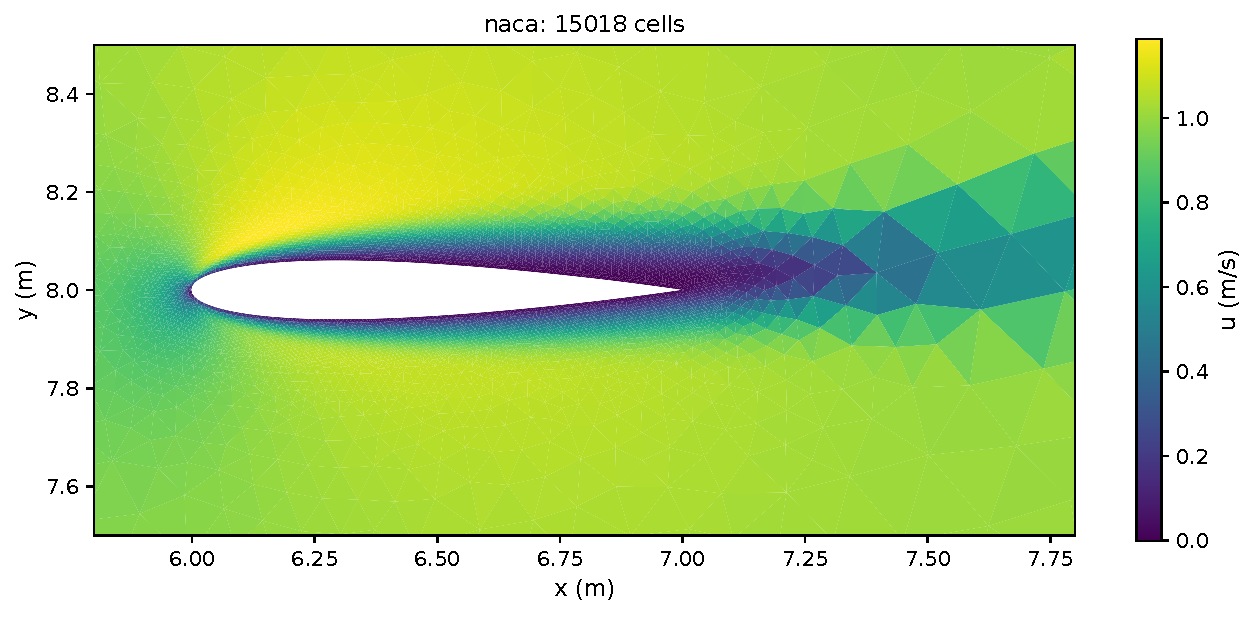
\includegraphics[width=.95\linewidth]{scale-1/figures/u-local.pdf}\caption{scale 1 figures u local}\end{figure}\begin{figure}[p]\centering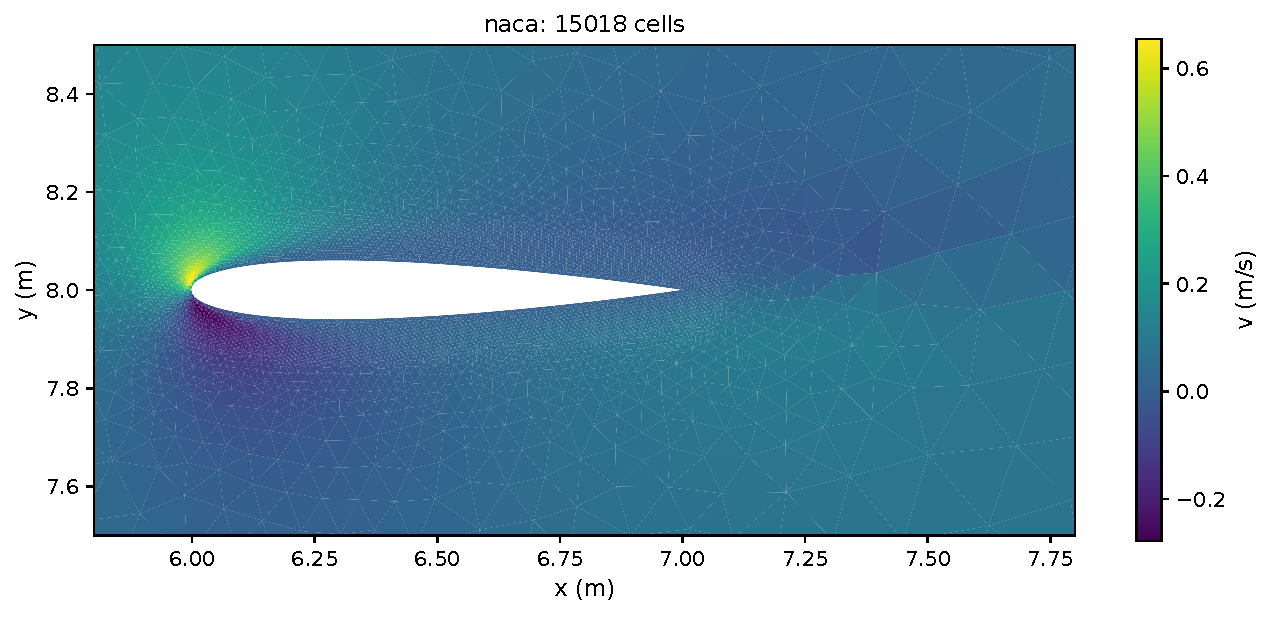
\includegraphics[width=.95\linewidth]{scale-1/figures/v-local.pdf}\caption{scale 1 figures v local}\end{figure}\begin{figure}[p]\centering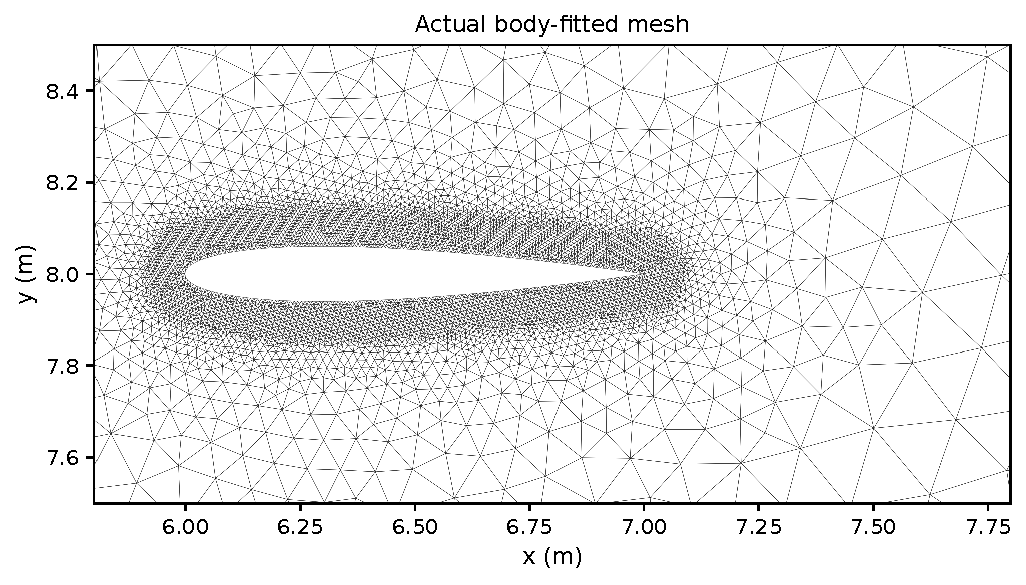
\includegraphics[width=.95\linewidth]{scale-1/figures/mesh-local.pdf}\caption{scale 1 figures mesh local}\end{figure}\begin{figure}[p]\centering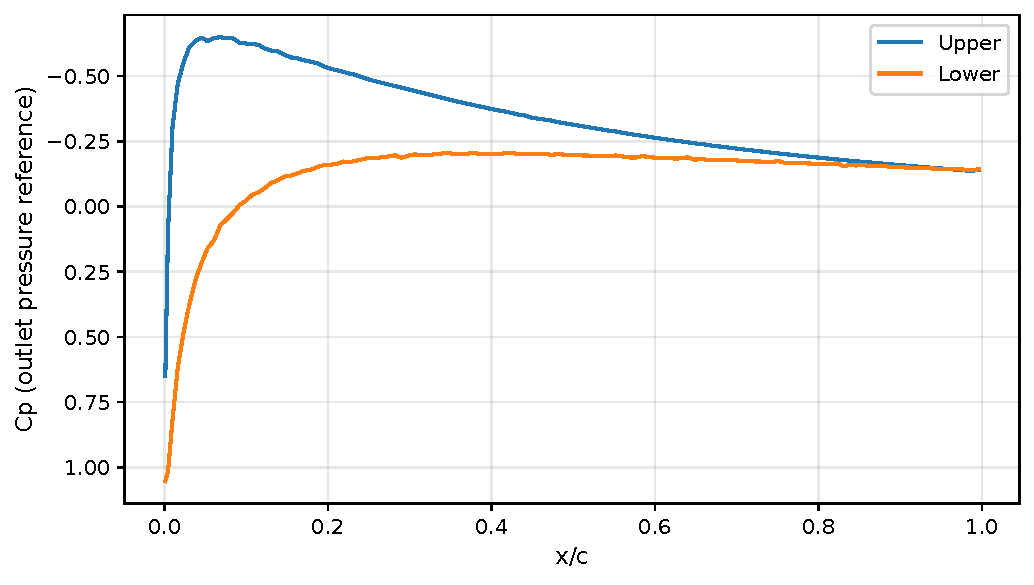
\includegraphics[width=.95\linewidth]{scale-1/figures/surface-pressure.pdf}\caption{scale 1 figures surface pressure}\end{figure}\begin{figure}[p]\centering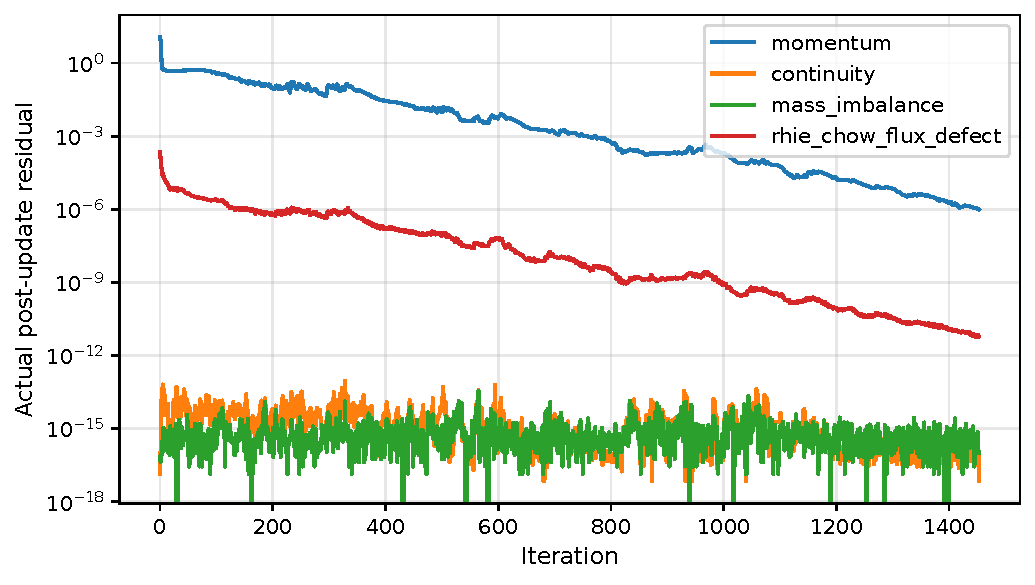
\includegraphics[width=.95\linewidth]{scale-1/figures/residuals.pdf}\caption{scale 1 figures residuals}\end{figure}\begin{figure}[p]\centering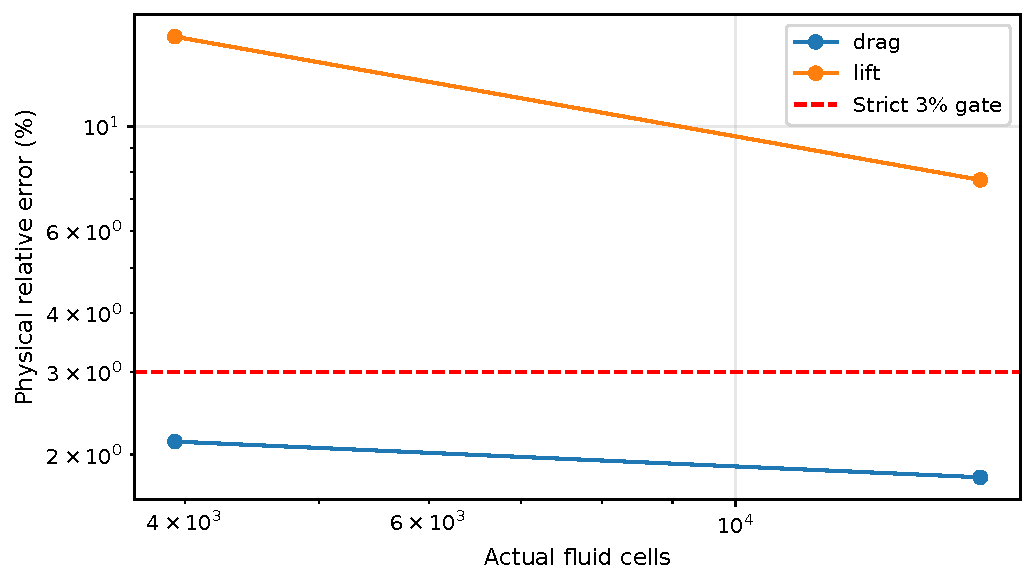
\includegraphics[width=.95\linewidth]{refinement.pdf}\caption{refinement}\end{figure}\end{document}
